\documentclass[20pt]{article}

\usepackage{geometry}
\usepackage{titlesec}
\usepackage{amsmath}
\usepackage{amssymb}
\usepackage[T1]{fontenc}
\usepackage{times}
\usepackage{tipa}
\usepackage{covington}
\usepackage{tikz}
\usepackage{tikz-qtree}

\setlength\parindent{0pt}
\newcommand{\ipa}[1]{\textipa{#1}}
\newcommand{\broad}[1]{/\ipa{#1}/}
\newcommand{\narrow}[1]{[ \ipa{#1} ]}
\newcommand{\english}[1]{$<$#1$>$}
\newcommand{\sk}[0]{{\kern 0.05em}}
\newcommand{\mk}[0]{{\kern 0.1em}}
\newcommand{\smallcapi}[0]{\sk\textsci\sk}
\newcommand{\openo}[0]{\sk O}
\newcommand{\feature}[1]{\ensuremath{\left[ \text{#1} \right]}}
\newcommand{\treeScale}[0]{0.7}
\newcommand{\rolesOpacity}[0]{0.7}
\newcommand{\rolesOne}[0]{$<$$\theta$$>$}
\newcommand{\rolesTwo}[0]{$<$$\theta$,$\theta$$>$}
\newcommand{\rolesThree}[0]{$<$$\theta$,$\theta$,$\theta$$>$}
\newcommand{\constituent}[2]{$[_{\text{#1}}$ #2$]$}

\titlespacing*{\section}{0pt}{0.7\baselineskip}{0.7\baselineskip}
\titleformat*{\section}{\large\bfseries}

\titleformat*{\subsection}{\normalsize\bfseries}

\begin{document}

\Large\textbf{Final Exam} \\
\normalsize
Alice McKean \\
\today

\section*{Part I}
\subsection*{Sentence 1}
\begin{tikzpicture}[scale=\treeScale, transform shape]
  \tikzset{every tree node/.style={align=center,anchor=north}}
  \Tree
  [.TP
    [.DP
      [.DP
        D\\The
        [.NP
          AP\\young
          NP\\actor
        ]
      ]
      [.D'
        D\\-s
        \node(DP-1-1){NP\\agent};
      ]
    ]
    [.T'
      T\\\feature{PAST}
      [.VP
        \node(DP-1-2){DP\\$t$};
        [.V'
          V\\got
          [.XP
            DP\\her
            [.X'
              X\\$\emptyset$
              [.DP
                D\\a
                [.NP
                  NP\\role
                  [.PP
                    P\\in
                    [.DP
                      D\\a
                      [.NP
                        AP\\popular
                        NP\\miniseries
                      ]
                    ]
                  ]
                ]
              ]
            ]
          ]
        ]
      ]
    ]
  ]
  \draw[->] (DP-1-2) to[bend left] (DP-1-1);
\end{tikzpicture}
\subsection*{Sentence 2}
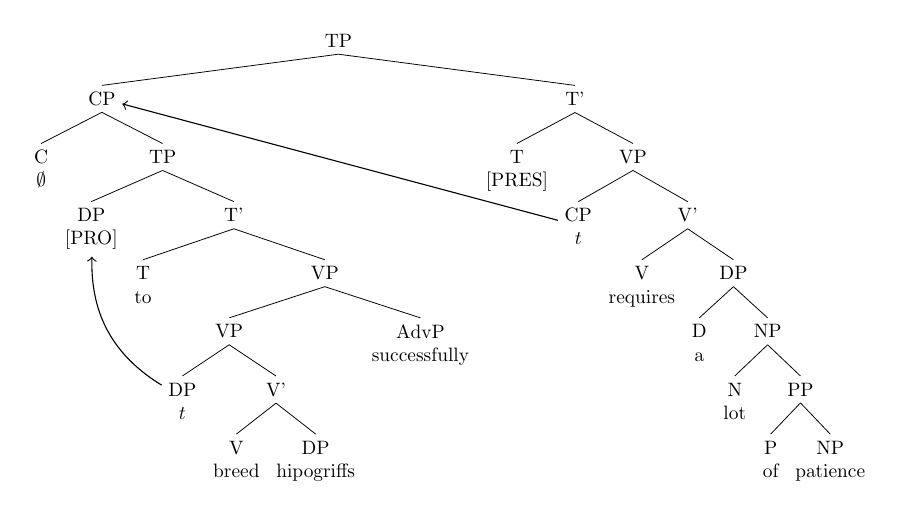
\begin{tikzpicture}[scale=\treeScale, transform shape]
  \tikzset{every tree node/.style={align=center,anchor=north}}
  \Tree
  [.TP
    [.\node(CP-1-1){CP};
      C\\$\emptyset$
      [.TP
        \node(DP-2-1){DP\\\feature{PRO}};
        [.T'
          T\\to
          [.VP
            [.VP
              \node(DP-2-2){DP\\$t$};
              [.V'
                V\\breed
                DP\\hipogriffs
              ]
            ]
            AdvP\\successfully
          ]
        ]
      ]
    ]
    [.T'
      T\\\feature{PRES}
      [.VP
        \node(CP-1-2){CP\\$t$};
        [.V'
          V\\requires
          [.DP
            D\\a
            [.NP
              N\\lot
              [.PP
                P\\of
                NP\\patience
              ]
            ]
          ]
        ]
      ]
    ]
  ]
  \draw[->] (DP-2-2) to[bend left] (DP-2-1);
  \draw[->] (CP-1-2) -- (CP-1-1);
\end{tikzpicture}
\subsection*{Sentence 3}
\begin{tikzpicture}[scale=\treeScale, transform shape]
  \tikzset{every tree node/.style={align=center,anchor=north}}
  \Tree
  [.TP
    [.DP
      D\\\feature{PROP}
      \node(DP-1-1){NP\\Louise};
    ]
    [.T'
      T\\\feature{PRES}
      [.VP
        [.VP
          \node(DP-1-2){DP\\$t$};
          [.V'
            V\\is
            AP\\anxious
          ]
        ]
        [.CP
          C\\for
          [.TP
            [.DP
              D\\the
              \node(DP-2-1){NP\\jury};
            ]
            [.T'
              T\\to
              [.VP
                \node(DP-2-2){DP\\$t$};
                [.V'
                  V\\find
                  [.XP
                    [.DP
                      D\\the
                      NP\\defendant
                    ]
                    [.X'
                      X\\$\emptyset$
                      AP\\innocent
                    ]
                  ]
                ]
              ]
            ]
          ]
        ]
      ]
    ]
  ]
  \draw[->] (DP-1-2) to[bend left] (DP-1-1);
  \draw[->] (DP-2-2) to[bend left] (DP-2-1);
\end{tikzpicture} \\
\subsection*{Sentence 4}
\begin{tikzpicture}[scale=\treeScale, transform shape]
  \tikzset{every tree node/.style={align=center,anchor=north}}
  \Tree
  [.CP
    \node(WH-1-1){DP\\Why};
    [.C'
      \node(C-1-1){C\\\feature{WH}\feature{Q}\\would};
      [.TP
        [.DP
          D\\the
          \node(DP-1-1){NP\\landlord};
        ]
        [.T'
          \node(T-1-1){T\\$t$};
          [.VP
            \node(DP-1-2){DP\\$t$};
            [.V'
              V\\want
              [.TP
                [.DP
                  D\\the
                  \node(DP-2-1){NP\\constable};
                ]
                [.T'
                  T\\to
                  [.VP
                    \node(DP-2-2){DP\\$t$};
                    [.V'
                      V\\arrest
                      [.XP
                        [.DP
                          D\\those
                          NP\\peasants
                        ]
                        [.X'
                          X\\$\emptyset$
                          \node(WH-1-2){DP\\$t$};
                        ]
                      ]
                    ]
                  ]
                ]
              ]
            ]
          ]
        ]
      ]
    ]
  ]
  \draw[->] (T-1-1) to[out=-90,in=0] (2, -6) to[out=180,in=-90] (C-1-1);
  \draw[->] (WH-1-2) to[out=-90,in=0] (10, -15) to[out=180,in=-90] (WH-1-1);
  \draw[->] (DP-1-2) to[bend left] (DP-1-1);
  \draw[->] (DP-2-2) to[bend left] (DP-2-1);
\end{tikzpicture}
\subsection*{Sentence 5}
\begin{tikzpicture}[scale=\treeScale, transform shape]
  \tikzset{every tree node/.style={align=center,anchor=north}}
  \Tree
  [.TP
    [.DP
      D\\That
      [.NP
        [.NP
          AP\\cranky
          [.NP
            AP\\old
            NP\\man
          ]
        ]
        [.\node(DP-1-1){PP};
          P\\in
          [.DP
            D\\the
            NP\\park
          ]
        ]
      ]
    ]
    [.T'
      T\\\feature{PRES}
      [.VP
        \node(DP-1-2){DP\\$t$};
        [.V'
          V\\seems
          [.CP
            C\\$\emptyset$
            [.TP
              \node(DP-2-1){DP\\$t$};
              [.T'
                T\\to
                [.VP
                  \node(DP-2-2){DP\\$t$};
                  [.V'
                    V\\enjoy
                    [.CP
                      C\\$\emptyset$
                      [.TP
                        \node(DP-3-1){DP\\\feature{PRO}};
                        [.T'
                          T\\\feature{GEN}
                          [.VP
                            \node(DP-3-2){DP\\$t$};
                            [.V'
                              V\\feeding
                              [.DP
                                D\\the
                                NP\\squirrels
                              ]
                            ]
                          ]
                        ]
                      ]
                    ]
                  ]
                ]
              ]
            ]
          ]
        ]
      ]
    ]
  ]
  \draw[->] (DP-1-2) to[bend left] (DP-1-1);
  \draw[->] (DP-2-1) to[bend left] (DP-1-2);
  \draw[->] (DP-2-2) to[bend left] (DP-2-1);
  \draw[->] (DP-3-2) to[bend left] (DP-3-1);
\end{tikzpicture} \\ 
\subsection*{Sentence 6}
\begin{tikzpicture}[scale=\treeScale, transform shape]
  \tikzset{every tree node/.style={align=center,anchor=north}}
  \Tree
  [.TP
    [.DP
      D\\\feature{PROP}
      \node(DP-1-1){NP\\Niall};
    ]
    [.T'
      T\\\feature{PRES}
      [.VP
        \node(DP-1-2){DP\\$t$};
        [.V'
          V\\wonders
          [.CP
            [.DP
              D\\which
              \node(WH-2-1){NP\\dishes};
            ]
            [.C'
              C\\\feature{WH}\feature{Q}
              [.TP
                [.DP
                  D\\\feature{PROP}
                  \node(DP-2-1){NP\\Luca};
                ]
                [.T'
                  T\\will
                  [.VP
                    \node(DP-2-2){DP\\$t$};
                    [.V'
                      V\\ask
                      [.TP
                        [.DP
                          D\\their
                          \node(DP-3-1){NP\\friends};
                        ]
                        [.T'
                          T\\to
                          [.VP
                            [.VP
                              \node(DP-3-2){DP\\$t$};
                              [.V'
                                V\\bring
                                \node(WH-2-2){DP\\$t$};
                              ]
                            ]
                            [.PP
                              P\\to
                              [.DP
                                D\\the
                                NP\\party
                              ]
                            ]
                          ]
                        ]
                      ]
                    ]
                  ]
                ]
              ]
            ]
          ]
        ]
      ]
    ]
  ]
  \draw[->] (DP-1-2) to[bend left] (DP-1-1);
  \draw[->] (DP-2-2) to[bend left] (DP-2-1);
  \draw[->] (DP-3-2) to[bend left] (DP-3-1);
  \draw[->] (WH-2-2) to[out=-90,in=0] (14, -18) to[out=180,in=-90] (WH-2-1);
\end{tikzpicture}

\section*{Part II}
\subsection*{Sentence 7}
\begin{tikzpicture}[scale=\treeScale, transform shape]
  \tikzset{every tree node/.style={align=center,anchor=north}}
  \Tree
  [.TP
    [.DP
      D\\\feature{PROP}
      \node(DP-1-1){NP\\Ari};
    ]
    [.T'
      T\\\feature{PAST}
      [.VP
        \node(DP-1-2){DP\\$t$};
        [.V'
          V\\tried
          [.CP
            C\\$\emptyset$
            [.TP
              \node(DP-2-1){DP\\\feature{PRO}};
              [.T'
                T\\to
                [.VP
                  \node(DP-2-2){DP\\$t$};
                  [.V'
                    V\\locate
                    [.DP
                      D\\a
                      [.NP
                        NP\\copy
                        [.PP
                          P\\of
                          [.DP
                            D\\that
                            NP\\manuscript
                          ]
                        ]
                      ]
                    ]
                  ]
                ]
              ]
            ]
          ]
        ]
      ]
    ]
  ]
  \draw[->] (DP-1-2) to[bend left] (DP-1-1);
\end{tikzpicture} \\

In Tree A the fragment "to locate a copy of that manuscript" does not form a
prepositional phrase. Consider the following sentence fragment test "Why did
Ari try?" with a response "to locate a copy of that manuscript". This is clearly
a bizarre way to respond to that question. Now change the WH element to what.
The question becomes "What did Ari try?" and the response "to locate a copy of
that manuscript" makes alot more sense. This shows that the response is a
complementizer phrase as shown in Tree B. Also consider replacing the same sentence
fragment with a pronoun. The full sentence becomes "Ari tried it" which is
clearly grammatical. Prepositional Phrases can not be replaced with pronouns.
Unfortunately both prepositional phrases and complementizer phrases can be
clefted and pseudo-clefted which renders theses tests inconclusive. A similar
argument applies to fronting. \\

The sentence fragment ``locate a copy'' does not form a verb phrase. Consider
the do so test ``Ari tried to do so of that manuscript''. This is clearly
ungrammatical. \\

The DP in Tree A ``a copy'' is not a DP. Consider replacing it with a pronoun.
The sentence ``Ari tried to locate it of that manuscript'' is terrible. Notice
that the fragment ``a copy of that manuscript'' does form a DP as shown in Tree
B. It passes the corresponding pronoun replacement test ``Ari tried to locate
it''. Consider coordinating ``a copy'' with another DP, for instance ``Ari tried
to locate a copy and replacement of that manuscript''. This sentence, while
grammatical, changes the semantics of the sentence. Now the copy could refer to
some non manuscript text. \\

Finally we turn to the non constituent and non category error. The subject of
the sentence ``Ari'' appears to move from two places simultaneously in Tree A.
This contradicts the fundamental definition of movement which is that a
constituent is copied from one place in the tree to another leaving \textit{one}
trace behind. A constituent may move again leaving another trace but importantly
it will be different then the original trace.

\section*{Part III}
For the rest of this final we document movement by superscripts and
co-indexation by subscripts in the interest of space.
\subsection*{Sentence 8}
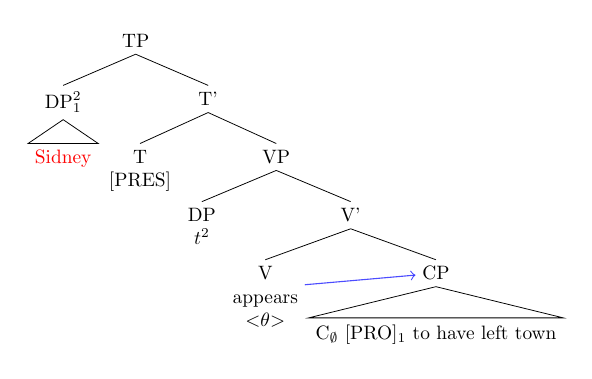
\begin{tikzpicture}[scale=\treeScale, transform shape]
  \tikzset{every tree node/.style={align=center,anchor=north}}
  \Tree
  [.TP
    [.DP$^2_1$
      \edge[roof];
      {\color{red} Sidney}
    ]
    [.T'
      T\\\feature{PRES}
      [.VP
        DP\\$t^2$
        [.V'
          \node(V-1-1){V\\appears\\\rolesOne{}};
          [.\node(CP-1-1){CP};
            \edge[roof];
            {C$_{\emptyset}$ \feature{PRO}$_1$ to have left town}
          ]
        ]
      ]
    ]
  ]
  \draw[blue, opacity=\rolesOpacity, ->] (V-1-1) -- (CP-1-1);
\end{tikzpicture} \\

Sentence 8 is ungrammatical as it violates the theta criterion. The theta
criterion says that every argument must recieve one unique theta role and the
constituent ``Sidney'' does not recieve a theta role. This is because the theta
role assigner ``appears'' only has one theta role to assign. The indexation is a
red herring as pronouns can be non locally bound so it does not violate any
binding principles. 
\subsection*{Sentence 9}
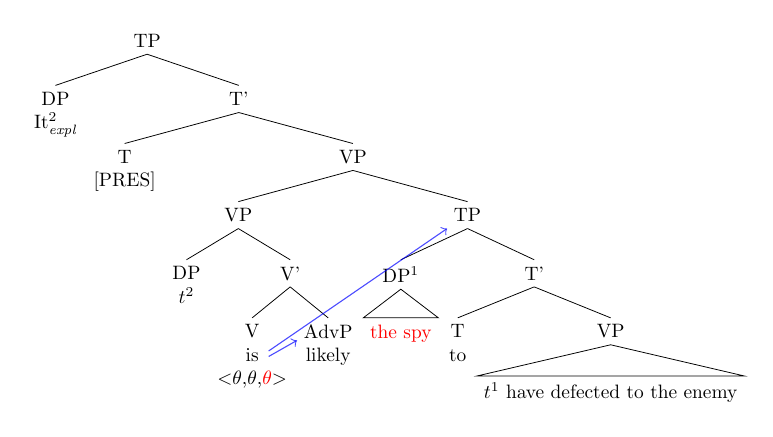
\begin{tikzpicture}[scale=\treeScale, transform shape]
  \tikzset{every tree node/.style={align=center,anchor=north}}
  \Tree
  [.TP
    DP\\It$_{\textit{expl}}^2$
    [.T'
      T\\\feature{PRES}
      [.VP
        [.VP
          DP\\$t^2$
          [.V'
            \node(V-1-1){V\\is\\$<$$\theta$,$\theta$,{\color{red} $\theta$}$>$};
            \node(AdvP-1-1){AdvP\\likely};
          ]
        ]
        [.\node(TP-1-1){TP};
          [.DP$^1$
            \edge[roof];
            {\color{red} the spy}
          ]
          [.T'
            T\\to
            [.VP
              \edge[roof];
              {$t^1$ have defected to the enemy}
            ]
          ]
        ]
      ]
    ]
  ]
  \draw[blue, opacity=\rolesOpacity, ->] ([xshift=0.3cm]V-1-1.center) -- (AdvP-1-1);
  \draw[blue, opacity=\rolesOpacity, ->] ([xshift=0.3cm,yshift=0.1cm]V-1-1.center) -- (TP-1-1);
\end{tikzpicture} \\

Firstly, the constituent ``the spy'' does not receive case so the sentence
violates the case filter. This is because ``to'' does not assign case and
the other case assigner ``is'' is not in a valid case assigning position.
Notice this analysis is also true if the embedded clause is wrapped
in a complementizer phrase. \\

Secondly the sentence violates the theta criterion as ``is'' has three theta
roles but only two roles are assigned. The theta criterion says that all theta
roles must be uniquely assigned.
\subsection*{Sentence 10}
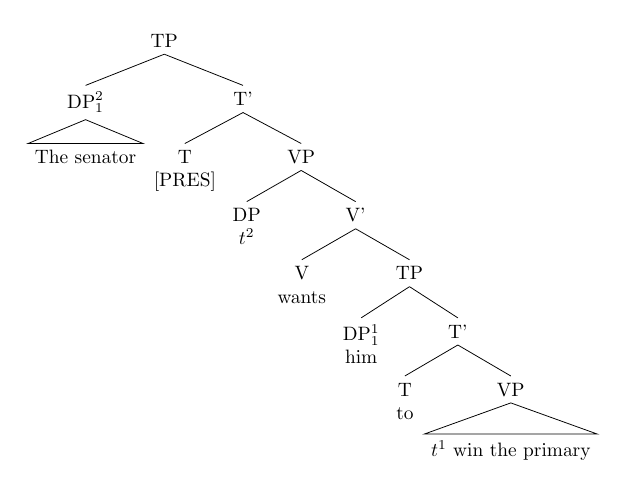
\begin{tikzpicture}[scale=\treeScale, transform shape]
  \tikzset{every tree node/.style={align=center,anchor=north}}
  \Tree
  [.TP
    [.DP$^2_1$
      \edge[roof];
      {The senator}
    ]
    [.T'
      T\\\feature{PRES}
      [.VP
        DP\\$t^2$
        [.V'
          V\\wants
          [.TP
            DP$^1_1$\\him
            [.T'
              T\\to
              [.VP
                \edge[roof];
                {$t^1$ win the primary}
              ]
            ]
          ]
        ]
      ]
    ]
  ]
\end{tikzpicture} \\

First notice that this sentence exhibits exceptional case marking so the embedded clause is not wrapped in a
complementizer phrase. If the embedded clause was wrapped in a complementizer
phrase then ``him'' would not receive case. This analysis is critical to
understanding why this sentence is ungrammatical as the smallest binding domain
of ``him'' is the matrix clause. This is because the matrix clause contains both
the case assigner ``wants'' and the subject ``The senator''. Thus the sentence
is ungrammatical by principle B, a pronoun must be free in it's binding domain.
\subsection*{Sentence 11}
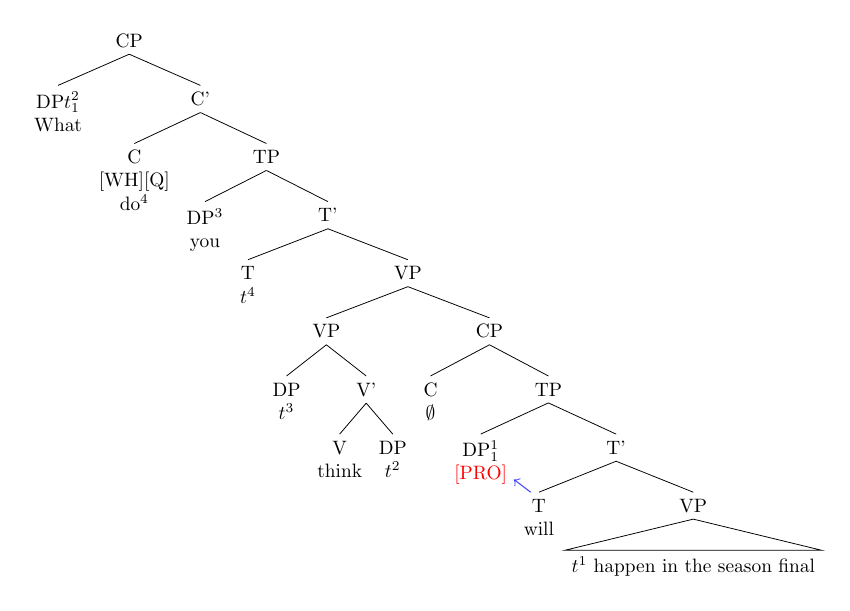
\begin{tikzpicture}[scale=\treeScale, transform shape]
  \tikzset{every tree node/.style={align=center,anchor=north}}
  \Tree
  [.CP
    DP$t^2_1$\\What
    [.C'
      C\\\feature{WH}\feature{Q}\\do$^4$
      [.TP
        DP$^3$\\you
        [.T'
          T\\$t^4$
          [.VP
            [.VP
              DP\\$t^3$
              [.V'
                V\\think
                DP\\$t^2$
              ]
            ]
            [.CP
              C\\$\emptyset$
              [.TP
                \node(DP-2-1){DP$^1_1$\\{\color{red} \feature{PRO}}};
                [.T'
                  \node(T-2-1){T\\will};
                  [.VP
                    \edge[roof];
                    {$t^1$ happen in the season final}
                  ]
                ]
              ]
            ]
          ]
        ]
      ]
    ]
  ]
  \draw[blue, opacity=\rolesOpacity, ->] (T-2-1) -- (DP-2-1);
\end{tikzpicture} \\
This sentence is a violation of the PRO Theorem which says that the
unpronounced pronoun can not receive case. The auxiliary ``will'' assigns
nominative case to the unpronounced pronoun.
\section*{Part IV}
\subsection*{Sentence 13}
\begin{tikzpicture}[scale=\treeScale, transform shape]
  \tikzset{every tree node/.style={align=center,anchor=north}}
  \Tree
  [.TP
    [.DP$^3$
      \edge[roof];
      {Rhonda}
    ]
    [.T'
      T\\\feature{PRES}
      [.VP
        DP\\$t^3$
        [.V'
          V\\wonders
          [.CP
            [.DP$^1$
              \edge[roof];
              {which picture of herself}
            ]
            [.C'
              C\\\feature{WH}\feature{Q}
              [.TP
                [.DP$^2$
                  \edge[roof];
                  {Brenda}
                ]
                [.T'
                  T\\\feature{PRES}
                  [.VP
                    DP\\$t^2$
                    [.V'
                      \edge[roof];
                      {likes $t^1$ best}
                    ]
                  ]
                ]
              ]
            ]
          ]
        ]
      ]
    ]
  ]
\end{tikzpicture} \\
In Sentence 13 both Rhonda and Brenda C-command herself but only Brenda
C-commands herself within herself's binding domain (pre-movement). Principle A
predicts that only Brenda should be allowed to co-index herself as Rhonda is not
in herself's binding domain before it moves. We could say that you may check
Principle A before or after movement.
\subsection*{Sentence 14}
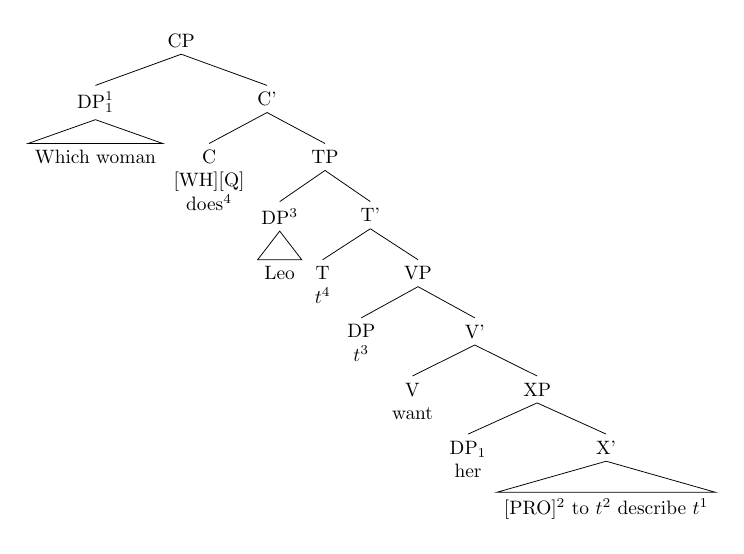
\begin{tikzpicture}[scale=\treeScale, transform shape]
  \tikzset{every tree node/.style={align=center,anchor=north}}
  \Tree
  [.CP
    [.DP$^1_1$
      \edge[roof];
      {Which woman}
    ]
    [.C'
      C\\\feature{WH}\feature{Q}\\does$^4$
      [.TP
        [.DP$^3$
          \edge[roof];
          {Leo}
        ]
        [.T'
          T\\$t^4$
          [.VP
            DP\\$t^3$
            [.V'
              V\\want
              [.XP
                DP$_1$\\her
                [.X'
                  \edge[roof];
                  {\feature{PRO}$^2$ to $t^2$ describe $t^1$}
                ]
              ]
            ]
          ]
        ]
      ]
    ]
  ]
\end{tikzpicture} \\
``Which woman'' is a R-expression and Principle C tells us that R-expressions
must be free. Before ``Which woman'' moves it is bound by ``her''. So if we
postulate that you check Principle C before movement the ungrammatically of the
sentence makes sense.
\subsection*{Sentence 15}
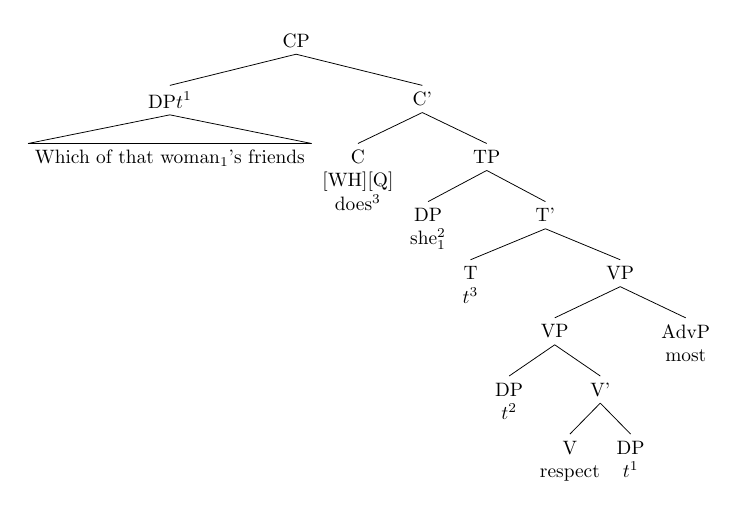
\begin{tikzpicture}[scale=\treeScale, transform shape]
  \tikzset{every tree node/.style={align=center,anchor=north}}
  \Tree
  [.CP
    [.DP$t^1$
      \edge[roof];
      {Which of that woman$_1$'s friends}
    ]
    [.C'
      C\\\feature{WH}\feature{Q}\\does$^3$
      [.TP
        DP\\she$^2_1$
        [.T'
          T\\$t^3$
          [.VP
            [.VP
              DP\\$t^2$
              [.V'
                V\\respect
                DP\\$t^1$
              ]
            ]
            AdvP\\most
          ]
        ]
      ]
    ]
  ]
\end{tikzpicture} \\
This sentence presents a problem to the theory because it follows a similar
pattern to sentence 14. The R-expression ``woman'' is bound by the antecedent
``she'' before movement this is because ``she'' C-commands ``woman'' before it
moves.
\end{document}

